%%%%%%%%%%%%%%%%%%%%%%% file template.tex %%%%%%%%%%%%%%%%%%%%%%%%%
%
% This is a general template file for the LaTeX package SVJour3
% for Springer journals.          Springer Heidelberg 2010/09/16
%
% Copy it to a new file with a new name and use it as the basis
% for your article. Delete % signs as needed.
%
% This template includes a few options for different layouts and
% content for various journals. Please consult a previous issue of
% your journal as needed.
%
%%%%%%%%%%%%%%%%%%%%%%%%%%%%%%%%%%%%%%%%%%%%%%%%%%%%%%%%%%%%%%%%%%%
%
% First comes an example EPS file -- just ignore it and
% proceed on the \documentclass line
% your LaTeX will extract the file if required
\begin{filecontents*}{example.eps}
%!PS-Adobe-3.0 EPSF-3.0
%%BoundingBox: 19 19 221 221
%%CreationDate: Mon Sep 29 1997
%%Creator: programmed by hand (JK)
%%EndComments
gsave
newpath
  20 20 moveto
  20 220 lineto
  220 220 lineto
  220 20 lineto
closepath
2 setlinewidth
gsave
  .4 setgray fill
grestore
stroke
grestore
\end{filecontents*}
%
\RequirePackage{fix-cm}
%
%\documentclass{svjour3}                     % onecolumn (standard format)
%\documentclass[smallcondensed]{svjour3}     % onecolumn (ditto)
\documentclass[smallextended]{svjour3}       % onecolumn (second format)
%\documentclass[twocolumn]{svjour3}          % twocolumn
%
\smartqed  % flush right qed marks, e.g. at end of proof
%
\usepackage{graphicx}
\usepackage{float}
\usepackage{amsmath}
%\usepackage{algorithm, algpseudocode}
\usepackage{algorithm}
\usepackage{algorithmic}
%\usepackage[]{algorithm2e}
\usepackage{url}
%\usepackage[noend]{algorithmic}
%\usepackage[english]{babel} 
%
% \usepackage{mathptmx}      % use Times fonts if available on your TeX system
%
% insert here the call for the packages your document requires
%\usepackage{latexsym}
% etc.
%
% please place your own definitions here and don't use \def but
% \newcommand{}{}
%
% Insert the name of "your journal" with
% \journalname{myjournal}
%
\begin{document}

\title{Fusion of IMU and Vision for Absolute Scale 
Estimation in Monocular SLAM%\thanks{Grants or other notes
%about the article that should go on the front page should be
%placed here. General acknowledgments should be placed at the end of the article.}
}
\subtitle{ENPM667 Midterm Project Report}

%\titlerunning{Short form of title}        % if too long for running head

\author{Harsh Kakashaniya         \and
        Rohitkrishna Nambiar%etc.
}

%\authorrunning{Short form of author list} % if too long for running head

\institute{Harsh Kakashaniya \at
				UID: \\
%              first address \\
%              Tel.: +123-45-678910\\
%              Fax: +123-45-678910\\
              \email{harshbk@umd.edu}           %  \\
%             \emph{Present address:} of F. Author  %  if needed
           \and
           Rohitkrishna Nambiar \at
           	UID: 115507944 \\
            \email{rohit517@umd.edu}
}

%\date{Received: date / Accepted: date}
\date{Submitted: 19th November 2018}
% The correct dates will be entered by the editor


\maketitle

\begin{abstract}
The fusion of inertial and visual data is widely used to improve an object’s
pose estimation. However, this type of fusion is rarely used to estimate further
unknowns in the visual framework. In this paper we present and compare two
different approaches to estimate the unknown scale parameter in a monocular
SLAM framework. Directly linked to the scale is the estimation of the object’s
absolute velocity and position in 3D. The first approach is a spline fitting task adapted
from Jung and Taylor and the second is an extended Kalman filter. Both methods
have been simulated offline on arbitrary camera paths to analyze their behavior and
the quality of the resulting scale estimation. We then embedded an online multi rate
extended Kalman filter in the Parallel Tracking and Mapping (PTAM) algorithm of
Klein and Murray together with an inertial sensor. In this inertial/monocular SLAM
framework, we show a real time, robust and fast converging scale estimation. Our approach does not depend on known patterns in the vision part nor a complex
temporal synchronization between the visual and inertial sensor.
\keywords{IMU vision fusion \and Absolute scale \and Monocular SLAM \and Kalman filter}
% \PACS{PACS code1 \and PACS code2 \and more}
% \subclass{MSC code1 \and MSC code2 \and more}
\end{abstract}
%\cleardoublepage
\newpage
\setcounter{tocdepth}{5}
\tableofcontents
\newpage
\listoffigures
\newpage
\section{Introduction}
\label{introduction}

This is a report of the paper titled \emph{Fusion of IMU and Vision for Absolute Scale Estimation in Monocular SLAM}~\cite{nutzi2011fusion}. On-board pose estimation is very useful for a variety of applications ranging from autonomous robotics to augmented reality. Pose estimation can be done using different sensors such as cameras and inertial measurement units (IMU). Simultaneous localization and mapping (SLAM) using a monocular camera can be used to get the trajectory of the camera and a map of the environment. But monocular cameras suffer from scale ambiguity causing the overall trajectory to drift making it unusable in real time. Using a stereo camera helps solve the scale ambiguity. IMUs on the other hand can be used to get the trajectory traveled by integrating the acceleration measurements over time. But this leads to highly inaccurate trajectory estimates. The estimate of the scale factor is essential to fuse both these measurements. This fusion helps us determine the unknown scale factor $\lambda$.    

In this paper~\cite{nutzi2011fusion}, two methods are presented for scale estimation. The first one is a spline fitting method by Jung and Taylor~\cite{jung2001camera}. The second is a multi rate Extended Kalman Filter(EKF). Both the approach have been simulated in MATLAB. 

This report is organized as follows. Section~\ref{hardware_setup} goes over the Camera and IMU setup, Section~\ref{imageFormation} covers the camera and image formation process, Section~\ref{mono_prob} goes over the scale estimation problem with monocular camera, Section~\ref{imusection} explains working of inertial measurement units, Section~\ref{Spline_1} outlines the spline fitting method with results, Section~\ref{ekf_section} covers Extended Kalman Filter and Section~\ref{slam} explains visual odometry, SLAM along with filter based and key-frame based methods.
\section{Hardware Setup}
\label{hardware_setup}

This section goes through the setup used in the research paper. USB uEye UI-122xLE fisheye camera was used as the vision input. The camera has a resolution of 752 × 480 and a frame rate up to 87 fps. Motion blur was minimized due to the high dynamic range and global shutter of the camera. VG400CC-200 solid state gyro which includes a tri-axial gyroscope and tri-axial accelerometer was used. It has an output frequency of 75 Hz with an input range of $\pm$10g and <1.25 mg resolution. The IMU outputs acceleration around its 3-axis along with yaw, pitch and roll.

% For one-column wide figures use
\begin{figure}[!htb]
% Use the relevant command to insert your figure file.
% For example, with the graphicx package use
  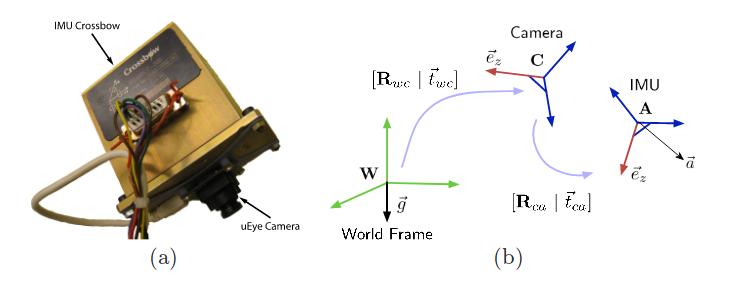
\includegraphics[width=\textwidth]{./figures/imucam.png}
% figure caption is below the figure
\caption{\textbf{a.} Camera/IMU setup. \textbf{b}. Frame transformations}
\label{fig:setup1}       % Give a unique label
\end{figure}
\section{Camera and image formation process}
\label{imageFormation}

To understand how a camera perceives the environment, it is necessary we understand the image formation process. For us humans, we “see” things when a light originating from a light source is reflected on an object and enters our eyes. A camera acts very much similar to the human eye. The earliest and first model of an optical camera is the pinhole camera which is a simple and highly accurate representation of our eye model. This is the simplest device to form an image of a 3D scene on a 2D surface. As seen in figure 1 rays of light enter the pinhole and forms an inverted image of the object. This is called perspective projection. As the image formed in the image place is inverted, we consider a virtual plane in front of the pinhole that acts as the image plane.  

% For one-column wide figures use
\begin{figure}[H]
% Use the relevant command to insert your figure file.
% For example, with the graphicx package use
  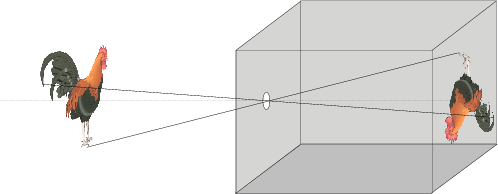
\includegraphics[width=\textwidth]{./figures/imageFormation.png}
% figure caption is below the figure
\caption{Please write your figure caption here}
\label{fig:1}       % Give a unique label
\end{figure}

Although the pinhole model is quite accurate, modern cameras have lenses. They help gather more light from a source leading to higher quality sharper images. Ignoring the internal diffraction, we assume thin lens equations for the imaging process. Every camera has a region of depths over which the scene is sharp. Modern cameras have variable apertures which help in focusing on objects at varying distances in the scene.  

Every camera has an intrinsic, extrinsic and distortion parameters that are important to understand for every application. These parameters are used to correct for lens distortion, measure objects in physical world and to determine the location of the camera in the real world. Camera calibration is the process of estimating these parameters specific to a given camera and application setup. Figure 2 demonstrates how the a real world 3D coordinate is related to a 2D pixel coordinate using the parameters mentioned above.

% For one-column wide figures use
\begin{figure}[H]
% Use the relevant command to insert your figure file.
% For example, with the graphicx package use
  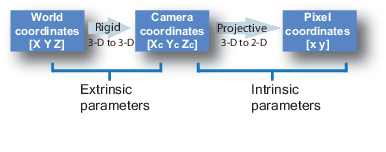
\includegraphics[width=\textwidth]{./figures/imageParams.png}
% figure caption is below the figure
\caption{Please write your figure caption here}
\label{fig:2}       % Give a unique label
\end{figure}

The extrinsic parameters relate the rotation R and translation t of the camera origin at the optical center to the world frame. The intrinsic parameters consists of the focal length given by fx and fy, the optical center given by cx and cy and the skew coefficient s. The distortion parameters consists of radial and tangential distortion along the x and y direction respectively. The number of coefficients are decided based on the lense in consideration. Camera calibration techniques presented in [4] [5] and [6] are widely used in commercial and open source camera calibration tool boxes.
\section{What's wrong with monocular camera?}
\label{mono_prob}

As the name suggests a monocular camera is a camera with a single imaging sensor. In section X. we say that given a perfectly calibrated camera ie. with the intrinsic and extrinsic parameters known, we can measure size of objects in the real world. This however is not true for a single image taken from a monocular camera. When 3D objects are projected onto the image plane (2D), the depth information stored in the z-axis is lost. This can be seen in the example below. 

% For one-column wide figures use
\begin{figure}
% Use the relevant command to insert your figure file.
% For example, with the graphicx package use
  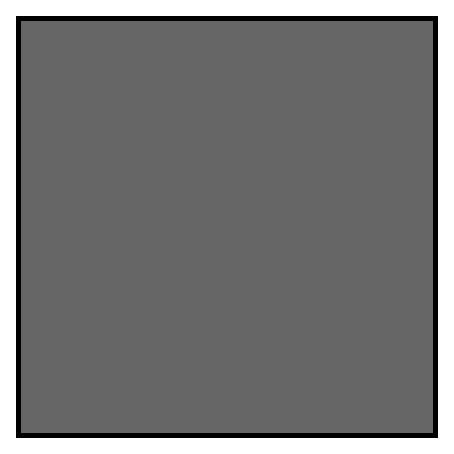
\includegraphics{example.eps}
% figure caption is below the figure
\caption{Monocular camera image coordinates}
\label{fig:3}       % Give a unique label
\end{figure}

As seen in the above diagram, irrespective of the location of the object in the real world, the size of the object in the image plane remains the same. Mathematically, this can be shown as 

\begin{equation}
\frac{y}{f}=\frac{y_1}{z_1+f}=\frac{y_2}{z_2+f}
\end{equation}

Where $f$ is the focal length of the camera. The title of the paper mentions scale estimation. In the context of SLAM which will be covered in the next section, scale is a term used to denote the factor by which the computed trajectory by a SLAM algorithm needs to be multiplied/scaled to make it equal to the ground truth. For example, if the measured distance is 2m, whereas the ground truth is 4m, the scale value would be 2. This is an area of active research and the community has come up with different techniques to solve this problem. As the title suggests, we would be talking about the fusion of IMU and Vision for solving this challenge.

\section{Spline Fitting Method}
\label{Spline_1}

In this paper there are 2 methods of fusing IMU data and Monocular camera. First of which is spline fitting using scale factor with the data of IMU and Monocular camera. Depending on the reliability of the data from both sources to estimate distance.So here we did simulation of whole system with arbitrary value of data considering linear moment of robot with noisy data. These simulations can be seen in result section. With the matlab code. So initially theory behind curve fitting is explained to have a algebraic background of types of curve fitting and their applications.We use spline in curve fitting because we get discrete data from sensors and camera but tracing spline helps for interpolation and extrapolation to have continuous high probability data of path.

Spline is fitted on the data points which is output of sensor in our case. Spline fitting also helps in reducing error due to noise. For Improving accuracy we can increase number of spline but this will also result into increase in computation. So we have to trade off between accuracy and computation.
Spline fitting is useful to give smooth curve .N degree spline may has N-1 curves in its shape. So if spline has X3 term that means it can have 2 curves in its spline.Ideal method to cover n points in a plan is by tracing nth order spline which will result into zero error. So spline will pass through all the points and will have a general equation as

\begin{equation}
\ A_{0} +A_{1}X +A_{2}X^{2}+A_{3}X^{3} + ... + A_{n}X^{n} = Y
\end{equation} 

This problem then converts in simple Ax = B form. we can get values of n terms by plugging in n points values.

Where

\begin{equation}
A = 
\begin{pmatrix}
  1 & X_{1} & X_{1}^{2} & \cdots & X_{1}^{n} \\
  1 & X_{2} & X_{2}^{2} & \cdots & X_{2}^{n} \\
  1 & X_{3} & X_{3}^{2} & \cdots & X_{3}^{n} \\
  : & :     &     :     & \cdots &    :      \\
  1 & X_{n} & X_{n}^{2} & \cdots & X_{n}^{n} \\
 \end{pmatrix}
B = 
\begin{pmatrix}
  A_{0} \\
  A_{1} \\
  A_{2} \\
  : 	\\
  A_{n} \\
 \end{pmatrix}
 C = 
\begin{pmatrix}
  Y_{0} \\
  Y_{1} \\
  Y_{2} \\
  : 	\\
  Y_{n} \\
 \end{pmatrix}
\end{equation}

But for practical applications we use other methods and do not plot n degree spline as it is computationally expensive .Secondly if there is more noise in system it will give wrong results. 
For practical application there are 3 kinds of spline fitting according to the application:-

\subsection{Types of curve fitting}
\subsubsection{Maximum error}
This is the method where spline is fit in a way where the point with maximum error is reduced and curve move towards the outlier point. If there exist in order to reduce maximum error of a point. This on the other hand results into

\begin{figure}[!htb]
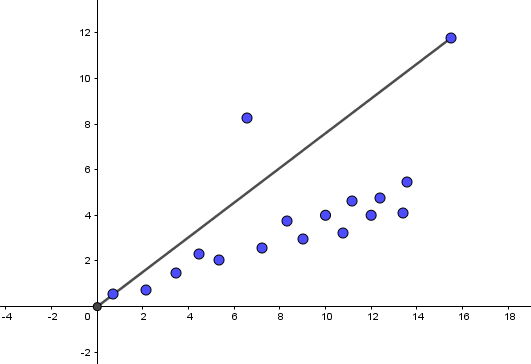
\includegraphics[width=\textwidth]{./figures/Maxerror.PNG}
\caption{Curve Fitting with Maximum error }
\end{figure}

\begin{equation}
E(f)=|max (f(xi)-yi)|  where i goes from 1 to left n
\end{equation}

Actually due to one outlier here line shifted in order to reduce maximum error. So this is not reliable process but is easy to compute.

\subsubsection{Average error}
This method is used to minimize average and fit the spline with minimum error conditions.

\begin{figure}[!htb]
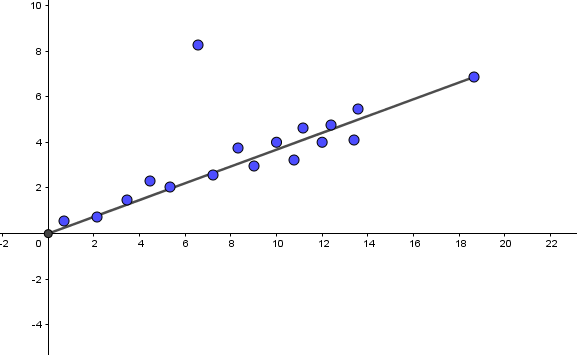
\includegraphics[width=\textwidth]{./figures/average.PNG}
\caption{Curve Fitting with Average error }
\end{figure}

\begin{equation}
E(f)=\frac{1}{n}*\Sigma|f(x_k)-Y_k| 
\end{equation}

Actually due to one outlier here line shifted in order to reduce maximum error. So this is not reliable process but is easy to compute.

\subsubsection{RMS (Least square method)}
This is the most efficient method to minimize the error this is also called as least square method.
Hence this is mostly used in curve fitting.
We have also created an algorithm with the help of same type of curve fitting.

\begin{figure}[!htb]
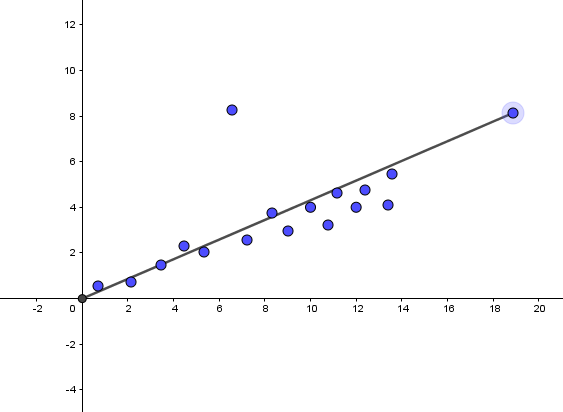
\includegraphics[width=\textwidth]{./figures/RMS.PNG}
\caption{Curve Fitting with RMS error }
\end{figure}

\begin{equation}
E(f)={\lbrace\frac{1}{n}*\Sigma|f(x_k)-Y_k|\rbrace}^\frac{1}{2} 
\end{equation}

\subsection{IMU Reading}
As we don’t have real IMU lets simulate virtual readings for this we took X, Y, Z as a function on time 

\begin{equation}
\label{For_x}
X_1=A_y t^2+B_y t +C_x
\end{equation}

\begin{equation}
Y_1=A_y t^2+B_y t +C_y
\end{equation}

\begin{equation}
Z_1=A_z t^2+B_z t +C_z
\end{equation}

With this treatment we will add some random noise to all the terms so that the data can be similar to what we obtain form IMU.

\begin{equation}
noise=A*(rand(1,n)-0.5)
\end{equation}

So our noise will range from -A/2 to A/2.
As function is rand() so it will change for every point.

\begin{equation}
X=X_1+noise
\end{equation}

\begin{equation}
Y=Y_1+noise
\end{equation}

\begin{equation}
Z=Z_1+noise
\end{equation}
We also took some random points of camera pose. And provided our system with data set.
Proof of Least square method in our case:
Let’s consider optimization of X first.
 
From equation \eqref{For_x} we have

Here $A$, $B$, $C$ are known
We have data set of X with respect to t
To calculate error in RMS we have
 
\begin{equation} 
 Error_x={\lbrace\displaystyle\sum_{i=1}^{n}(|X_i-(A_xt_i^2+B_x t_i +C_x)|)^2\rbrace}^\frac{1}{2} 
\end{equation}


When we differentiate some quantity and equate it to zero it goes to either minima or maxima
And if double derivative is positive it goes to minima.

So in this case if we take partial derivatives of error with respect to Ax , Bx , Cx

\begin{equation} 
 \frac{\partial Error_x}{\partial A_x} = {\lbrace\displaystyle\sum_{i=1}^{n}2(|X_i-(A_xt_i^2+B_x t_i +C_x)|)\rbrace}({-t_i^2})
\end{equation}

\begin{equation} 
\displaystyle\sum_{i=1}^{n}(|{-t_i^2}X_i+(A_x t_i^4+B_x t_i^3+C_x t_i^2)|) = 0
\end{equation}

\begin{equation} 
 \frac{\partial Error_x}{\partial B_x} = {\lbrace\displaystyle\sum_{i=1}^{n}2(|X_i-(A_xt_i^2+B_x t_i +C_x)|)\rbrace}({-t_i})
\end{equation}

\begin{equation} 
\displaystyle\sum_{i=1}^{n}(|{-t_i}X_i+(A_x t_i^3+B_x t_i^2+C_x t_i^1)|) = 0
\end{equation}

\begin{equation} 
 \frac{\partial Error_x}{\partial C_x} = {\lbrace\displaystyle\sum_{i=1}^{n}2(|X_i-(A_xt_i^2+B_x t_i +C_x)|)\rbrace}({-1})
\end{equation}

\begin{equation} 
\displaystyle\sum_{i=1}^{n}(|{-1}X_i+(A_x t_i^2+B_x t_i+C_x)|) = 0
\end{equation}

So we can compute matrix in such a way that the problem changes to 

Ax=B

Where, 

\begin{equation}
A = 
\begin{pmatrix}
  \Sigma t^4 & \Sigma t^3 & \Sigma t^2\\
  \Sigma t^3 & \Sigma t^2 & \Sigma t\\
  \Sigma t^2 & \Sigma t & \Sigma 1\\
 \end{pmatrix}
B = 
\begin{pmatrix}
  A_x \\
  B_x \\
  C_x \\
 \end{pmatrix}
 C = 
\begin{pmatrix}
  \Sigma X_i t ^2 \\
  \Sigma X_i t \\
  \Sigma X_i \\
 \end{pmatrix}
\end{equation}

From this equation we can calculate X matrix.Similarly,We can get X matrix of Y and Z axis.

\begin{equation}
A = 
\begin{pmatrix}
  \Sigma t^4 & \Sigma t^3 & \Sigma t^2\\
  \Sigma t^3 & \Sigma t^2 & \Sigma t\\
  \Sigma t^2 & \Sigma t & \Sigma 1\\
 \end{pmatrix}
B = 
\begin{pmatrix}
  A_y \\
  B_y \\
  C_y \\
 \end{pmatrix}
 C = 
\begin{pmatrix}
  \Sigma Y_i t ^2 \\
  \Sigma Y_i t \\
  \Sigma Y_i \\
 \end{pmatrix}
\end{equation}

\begin{equation}
A = 
\begin{pmatrix}
  \Sigma t^4 & \Sigma t^3 & \Sigma t^2\\
  \Sigma t^3 & \Sigma t^2 & \Sigma t\\
  \Sigma t^2 & \Sigma t & \Sigma 1\\
 \end{pmatrix}
B = 
\begin{pmatrix}
  A_z \\
  B_z \\
  C_z \\
 \end{pmatrix}
 C = 
\begin{pmatrix}
  \Sigma Z_i t ^2 \\
  \Sigma Z_i t \\
  \Sigma Z_i \\
 \end{pmatrix}
\end{equation}

By this treatment we converted given points into equation with least square method here we used condition of 

\begin{equation}
min
\begin{pmatrix}
  A_x t^2 + B_x t + C_x -\lambda_i X_c \\
  A_y t^2 + B_y t + C_y -\lambda_i Y_c \\
  A_z t^2 + B_z t + C_z -\lambda_i Z_c \\
 \end{pmatrix}^2
 \end{equation}
 
 Here in this formula we have different value of  for different spline according to accuracy of camera data and IMU reading.

\subsection{Results}
 
 In our case we simulated the results and found following outputs.
Plotting the second order curve for given data of IMU with just least square method. We get the following graph

\begin{figure}[!htb]
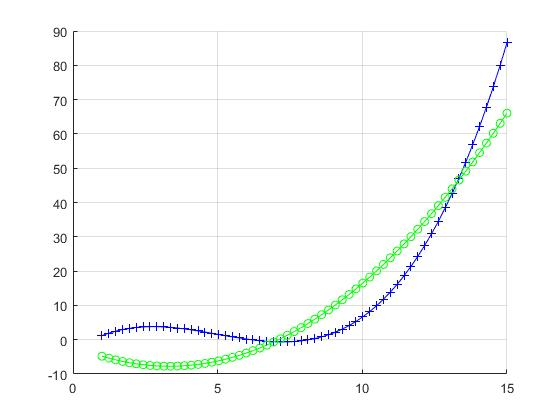
\includegraphics[width=\textwidth,height=7cm,keepaspectratio]{./figures/lsm.jpg}
\caption{In this case Blue is actual curve traced by IMU this are points with noise.And green is plotted curve. With least square method.}
\end{figure}

Then according to the paper we fused data of camera and IMU so we get following graph.

\begin{figure}[!htb]
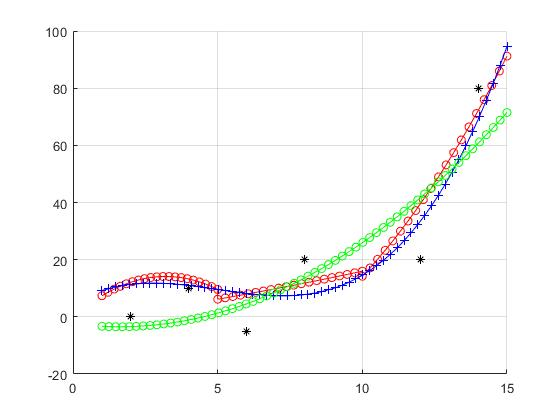
\includegraphics[width=\textwidth,height=7cm,keepaspectratio]{./figures/AllOutput.jpg}
\caption{Multiple spline fit}
\label{fig:multipleSpline}
\end{figure}

In Figure~\ref{fig:multipleSpline} we have 3 curved fitted as shown as red which gives better results and it also uses data of camera shown with black dots. So here according to the above formula scale factor of different section is different it is according to the quality of reading by camera.
For example, in our case 
\begin{equation}
\lambda_1=0.5 ,\lambda_2=0.5 ,\lambda_3=0.1
\end{equation}

In 3rd section camera readings were not accurate so taken into smaller scalar value. This camera data further improved the result. And we get minimum error and good fit. With the given spline fitting method.

So if we look into different of error with traditional Least square method with Jung and Taylor method. It gives good results. Almost we get the same curve.

\begin{figure}[!htb]
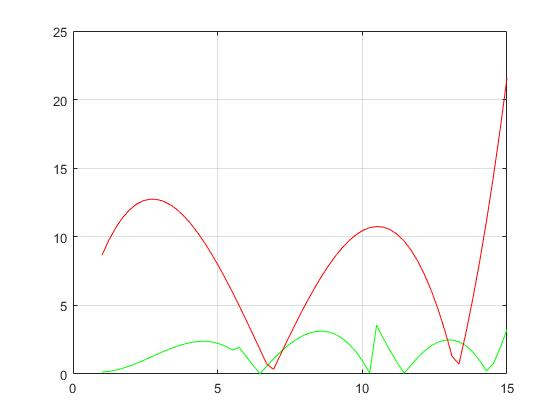
\includegraphics[width=\textwidth,height=7cm,keepaspectratio]{./figures/ErrorC.jpg}
\caption{\textbf{a}. Red curve for method with one curve and least square method. 
\textbf{b}. Green curve is using the given method by Jung and Taylor.}
\label{fig:errorc1}
\end{figure}

The graph in Figure 12 has error comparison with and without Jung and Taylor method of split curve fitting and scaling camera input.
So it is better to follow the given first method in the paper. It results into considerable reduction in error which is clearly seen in graph.

With the same approach we can optimize and plot spline in 3 Dimension so when we use this algorithm for 3D space we get the following result where we get an second order optimized curve. we also included considerable noise and tested our algorithm.
  
\begin{figure}[H]
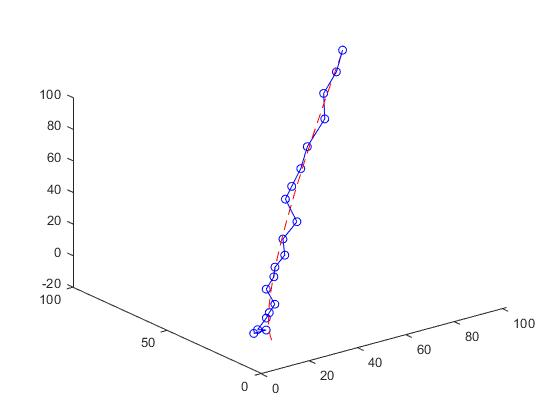
\includegraphics[width=\textwidth,height=7cm,keepaspectratio]{./figures/3DCurve.jpg}
\caption{Actual 3D path with noise vs Optimized spline fit}
\label{fig:errorc1}
\end{figure}
%\section{Extended Kalman Filter}
\label{Spline_1}

\subsection{Introduction}
In estimation theory, the extended Kalman filter (EKF) is the nonlinear version of the Kalman filter which linearizes about an estimate of the current mean and covariance. In the case of well defined transition models, the EKF has been considered to estimate the state. 
in this system we have a state and an observer these are given by equation.
$ X=AX +BU + W_d $  and $ Y=CX + W_n $
In this $ W_d $ is disturbance and $ W_n $ is the noise by sensor.
So Kalman filter is used judges between data be disturbance and noise.

If $W_d >> W_n$ that means disturbance amount is higher than noise hence state estimation can rely more on sensor data for mapping than on previous state. And sensor is more reliable.

if $W_n >> W_d$ that means noise amount is higher than disturbance hence state estimation can rely more on previous plot data for mapping than on sensor. And state is more reliable than sensor.

So according in paper we learned that non-linear system is defined as.



\begin{algorithm}
\caption{Kalman filter algorithm}\label{alg-gd}
\begin{algorithmic}[1]
\STATE Kalman Filter \({(\mu_{t-1},\Sigma_{t-1},u_t,z_t)}\)
\STATE \( {\mu_{t}}=A_t \mu_{t-1} + B_t u_t \)
\STATE \( \Sigma_{t}=A_t \Sigma_{t-1} A_t^T +R_t\)
\STATE \( K_t = \Sigma_{t} C_t(C_t^T \Sigma_{t}C_t^T+Q_t)^{-1}\)
\STATE \( \mu_{t}=\mu_{t}+K_t(z_t-C_t \mu_t) \)
\STATE \(\Sigma_{t}=(I-K_t C_t)\Sigma_{t}\)
\STATE return \( \mu_t ,  \Sigma_t \)
\end{algorithmic}
\end{algorithm}

So now lets take non-linear state equation as follows

\begin{equation}
\overrightarrow{z}_{k+1}= \overrightarrow{f}_k (\overrightarrow{z}_k) + v_k 
\end{equation}

\begin{equation} 
\begin{pmatrix}
  \overrightarrow{x}_{k+1} \\
  \overrightarrow{v}_{k+1} \\
  \overrightarrow{a}_{k+1} \\
  \overrightarrow{\lambda}_{k+1} \\
 \end{pmatrix}
 =
 \begin{pmatrix}
  I_3 & \frac{T}{\lambda}I_3  & \frac{T^2}{2 \lambda} I_3 & 0\\
  0 & I_3 & T I_3 & 0 \\
  0 & 0 & I_3 & 0 \\
  0 & 0 & 0 & 1\\
 \end{pmatrix} 
\begin{pmatrix}
\overrightarrow{x}_{k} \\
  \overrightarrow{v}_{k} \\
  \overrightarrow{a}_{k} \\
  \overrightarrow{\lambda}_{k} \\
 \end{pmatrix}
\end{equation}

where $x_k+1$ is the position without scale of the IMU/Camera and $v_{k+1}$ , $a_k+1$ are the velocity and acceleration of the IMU/Camera in metric unit [m]. $ν_k$ is the gaussian process noise. 
Every vector in $z_k$ is resolved in the world frame W. Note that we do not
include the orientation information in the model nor use it as a measurement in order. to keep the algorithm simple and fast. On each acceleration measurement we do the conversion from the inertial to the world frame by using a zero order hold  of the unfiltered attitude measurement returned by the visual SLAM framework. As we work in a middle size environment with enough loops we assume negligible drift in the SLAM map and assume thus highly accurate attitude estimation from the visual SLAM framework. The model in its linearized form yields,

\begin{equation} 
F_k= 
 \begin{pmatrix}
  I_3 & \frac{T}{\lambda}I_3  & \frac{T^2}{2 \lambda} I_3& -\frac{T}{ \lambda^2} I_3 - \frac{T^2}{ 2 \lambda^2} I_3\\
  0 & I_3 & T I_3 & 0 \\
  0 & 0 & I_3 & 0 \\
  0 & 0 & 0 & 1\\
 \end{pmatrix} 
\end{equation}

For fusion implementation we consider the measurements in different observation
vectors. For a multi rate filter, as it is in our case, the literature suggests two solutions. One would be using a (higher order) hold to synchronize the different measurements. Another is to weight the uncertainty of the measurement according to its temporal occurrence. We claim no certainty at all if no
measurement is available (i.e. the measurement noise variance is infinite). Thus the update equations simplify to improve results. A more complex weighting function (i.e. exponential decay in time) could also be applied, however, at the cost of speed. The measurement updates for the vision and the IMU yields (‘V’ and ‘I’ denotes Vision and IMU)

The innovation done by authors in for the vision part is,
\begin{equation}
K_{V,k}=P_k^- H_{V,k}^T (H_{V,k} P_k H_{V,k}^T +R_v)^{-1}
\end{equation}
\begin{equation}
\overrightarrow{z}_{k}=\overrightarrow{z}_{k}+K_{V,k}(\overrightarrow{x}_{SLAM}-H_{V,k} \overrightarrow{z}_{k})
\end{equation}
\begin{equation}
P_k=(I-K_{V,k} H_{V,k}) P_k^-
\end{equation}

The innovation for by authors in the IMU part is,
\begin{equation}
K_{I,k}=P_k^- H_{I,k}^T (H_{I,k} P_k H_{I,k}^T +R_I)^{-1}
\end{equation}
\begin{equation}
\overrightarrow{z}_{k}=\overrightarrow{z}_{k}+K_{I,k}(\overrightarrow{x}_{IMU}-H_{I,k} \overrightarrow{z}_{k})
\end{equation}
\begin{equation}
P_k=(I-K_{I,k} H_{I,k}) P_k^-
\end{equation}

The two matrices $R_I$ , $R_V$ are the noise covariance matrices for the vision and IMU measurement inputs $x_{SLAM}$ , $a_{IMU}$ which are resolved in the world frame W.
The vector $x_{SLAM}$ is the position without scale obtained from the vision algorithm(SLAM). The IMU measurement $a_{IMU}$ needs special attention, because significant errors arise in the conversion from the raw IMU output.
\begin{equation}
\overrightarrow{a}_{w}=R_{wc}R_{ca} (\overrightarrow{a}_a - \overrightarrow{b})-\overrightarrow{g}_w
\end{equation}


\section{Simultaneous Localization and Mapping}
\label{slam}

In this section, we cover SLAM, and the different concepts related to SLAM such as Visual Odometry. We then explore the two different approaches to SLAM mentioned in the paper. We briefly cover filter based SLAM called Extended Kalman Filter SLAM (EKFSLAM) and a key-frame based SLAM called Parallel Tracking and Mapping (PTAM)~\cite{klein2007parallel}. Simultaneous Localization and Mapping (SLAM) is a technique for estimating the motion of the robot and reconstructing the map/structure of the unknown environment. SLAM using only visual information only is specifically referred to as visual SLAM (vSLAM). The SLAM problem can be stated as follows:\\

\textbf{\emph{How can a body navigate in a previously unknown environment while constantly building and updating a map of its workspace using onboard sensors only?} ~\cite{chli2017}}\\

From the problem statement above, we notice that the robot has no a priori knowledge of the workspace or environment that it is in. This makes SLAM a very challenging problem in probabilistic robotics. This is also referred to as a chicken-egg problem in that we need to map the environment to get an accurate pose, but at the same time we also need an accurate pose to build a correct map. Therefore, it is an iterative process of estimating pose and building a map simultaneously. Accurate pose estimation is critical for many applications in computer vision, autonomous robotics and augmented reality.
  

% For one-column wide figures use
\begin{figure}
% Use the relevant command to insert your figure file.
% For example, with the graphicx package use
  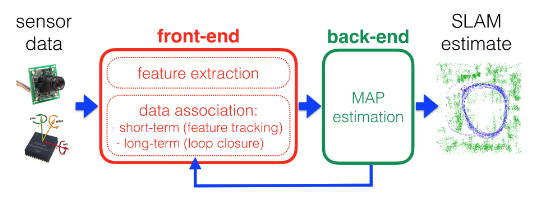
\includegraphics[width=\textwidth]{./figures/slam_model.png}
% figure caption is below the figure
\caption{SLAM architecture}
\label{fig:slammodel}       % Give a unique label
\end{figure}

From Fig ~\ref{fig:slammodel} we see that a typical SLAM system consists of a front-end and a back-end. The front-end is responsible for feature extraction while the back-end is responsible for MAP estimation. Both the methods (EKFSLAM \& PTAM) are feature based implementations. 

\subsection{Visual Odometry}

Odometry is the technique of estimating the position of a robot over time using sensors such as cameras,  wheel encoders or any sensor measuring relative movement. Compared to SLAM which maintains a global consistent map, visual odometry (VO) maintains a local consistent map optimized over the last n frames. A generalized VO pipeline can be summarized as follows

% For one-column wide figures use
\begin{figure}[!htb]
% Use the relevant command to insert your figure file.
% For example, with the graphicx package use
  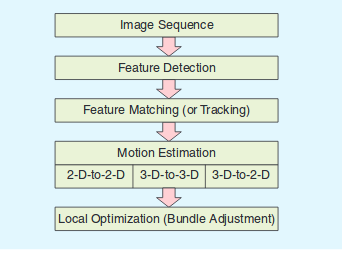
\includegraphics[width=\textwidth]{./figures/vo.png}
% figure caption is below the figure
\caption{Generalized Visual Odometry Pipeline}
\label{fig:vo}       % Give a unique label
\end{figure}

Different algorithms exist due to the different type of cameras available such as Stereo, Mono, RGB-D. As we use a monocular setup in our research paper, we would be going through the visual odometry algorithm from 2D to 2D correspondences for a monocular sensor. The algorithm is summarized as follows.

\begin{algorithm}
    \caption{Monocular Visual Odometry}
	\begin{algorithmic}[1]
		\STATE Capture a new image frame $I_k$
    	\STATE Extract and match features between frames $I_k$ and $I_{k-1}$
    	\STATE Compute the essential matrix $E$ from the matched feature points
    	\STATE Decompose $E$ into $R_k$ and $t_k$ to form $T_k$
    	\STATE Choose the correct $T_k$ matrix and scale $t_k$ accordingly from scale factor
    	\STATE Compute $C_k$ = $C_{k-1}*T_k$
    	\STATE Goto step 1.
	\end{algorithmic}
\end{algorithm}

Since we are using a monocular sensor, we always compare the image $I_k$ captured at time instant $k$ with the image $I_{k-1}$ capture at time instant $k-1$. In a stereo setup, we would compare images from the left and right part of the stereo. Once an image is captured, we compute the features for image $I_k$ and $I_{k-1}$. In the feature detection step, the image is searched for key-points called features  which are likely to be present in successive images. Features can be defined as image patterns that differ from its immediate neighborhood in terms of intensity, color and texture. There exist a variety of feature detectors in literature which vary in performance and properties. Some of the properties of feature detectors are rotation, scale and affine invariant, repeatability, localization accuracy, robustness and efficiency.  Heitanen et al. present a comparison of feature detectors and descriptors for object class matching in~\cite{hietanen2016comparison}. Once we detect features, we then need to compute a descriptor such that features detected in two images can be compared with each other. The easiest approach would be to form a patch of pixels and compare using a sum of squared distances (SSD) or normalized cross correlation (NCC) metric. Such descriptors are not invariant to any of the above mentioned properties and perform poorly in practical applications. One of the popular descriptors called SIFT~\cite{lowe2004distinctive} uses gradient orientations as its descriptors. This forms a 128-element descriptor that is invariant to most of the above mentioned properties such as rotation, scale and illumination which makes it widely applicable in practical real-time applications. For extracting features from two images there are two paths with one being to detect and match features independently in two frames and the other being to track features in subsequent frames an example of which is a KLT Tracker~\cite{tomasi1991detection}. There are various methods employed to match features accurately such a RANSAC which stands for Random Sample Consensus and is used to remove outliers among feature matches. Once we detect and match features in $I_k$ and $I_{k-1}$, we calculate the essential matrix $E$ which describes the geometric relationship between two images. We can use Nister’s five point algorithm~\cite{nister2004efficient} or Longuet-Higgins eight point algorithm~\cite{longuet1981computer} to get the essential matrix $E$. Once we get the essential matrix $E$, we decompose it to extract the rotation and translation parts. Four different solutions are obtained of which the correct pair can be found out by triangulation. The solutions are given as

\begin{equation}
	R = U(\pm W^T)V^T
\end{equation}

\begin{equation}	
	t = U(\pm W^T)SV^T
\end{equation}

where R is the rotation matrix and t is the translation vector. 

\subsection{EKFSLAM}

\subsection{Parallel Tracking and Mapping (PTAM)}
\label{ptamtheory}

PTAM is a SLAM system specifically designed to track a hand-held camera in a small AR workspace. For real-time operation, PTAM splits the tracking and mapping threads into two separate tasks running in parallel. The tracking thread robustly tracks hand-held motion and the mapping thread produces a 3D map of the features. Although developed specific to AR applications, the concept of running operations on multiple threads was incorporated into future SLAM algorithms. 

The map consists of a collection of key-points/features that are located in a world frame $W$. They are represented in the homogeneous form. The map also contains key-frames which a instances of the frames taken from the hand-held camera. Each point is stored with a source key-frame. Unlike earlier methods which process each and every frame, this method only processes frames when there is sufficient information. Thus incremental mapping is replaced with a more computationally expensive batch method called bundle adjustment. 

The tracking algorithm can be summarized as follows.

\begin{algorithm}
    \caption{PTAM - Tracking Algorithm}
    \begin{algorithmic}[1]
		\STATE A new frame is captured and a prior pose estimate is generated from motion model.
    	\STATE Map points are projected into the image based on prior pose. 
    	\STATE Small number of features (50) are searched in the image.
    	\STATE The camera pose is updated from the feature matches.
    	\STATE Large number of points is re-projected and searched in the image.
    	\STATE Final pose estimate is computed from all matched found. 
    	\STATE Goto step 1.
    \end{algorithmic}
\end{algorithm}

PTAM is initialized by a lateral offset movement of the hand-held camera. This can be assumed as a stereo image for starting the mapping. The initial map is constructed using the 5 point algorithm~\cite{nister2004efficient} with arbitrary scale. As the camera moves, the key-frames increase from an initial two. Here, we only add key-frames if the tracking quality is good and a minimum of twenty frames has passed from the last keyframe. Bundle adjustemnt is iteratively performed to adjust the map based on a cost function. The mapping algorithm can then be summarized as.

\begin{algorithm}
    \caption{PTAM - Mapping Algorithm}
	\begin{algorithmic}[1]
		\REQUIRE \mbox{Stereo Initialization}
		\IF {New Keyframe}
			\STATE Update key-frame
			\STATE Integrate key-frame
			\STATE Add new features
		\ELSIF {Locally Converged}
			\IF {Globally Converged}
				\STATE Update data association
			\ELSE
				\STATE Global bundle adjust
			\ENDIF
		\ELSE
			\STATE Locally bundle adjust
		\ENDIF
		\STATE Sleep 5ms
		\STATE Goto step 1.
	\end{algorithmic}
\end{algorithm}

Finally when compared with Filter based SLAM, PTAM can handle thousands of features by splitting the tracking and mapping onto different threads on the CPU. We see that SLAM algorithms built now-a-days have used this philosophy to great success. 

\subsection{Results}
\subsubsection{Simulated and Real Data}

In the paper, the Kalman filter was simulated offline with simulated data from the spline fitting section. The two inputs to the Kalman filter were the position from the vision sensor and acceleration from the IMU. Three different approaches were taken. The first method is same as Eq. 7, the second method only uses the Z-axis which gives the states as $[\overrightarrow{x}_z, \overrightarrow{\nu}_z, \overrightarrow{\alpha}_z, \lambda]$ and the third uses only the X and Y-axis. 

% For one-column wide figures use
\begin{figure}
% Use the relevant command to insert your figure file.
% For example, with the graphicx package use
  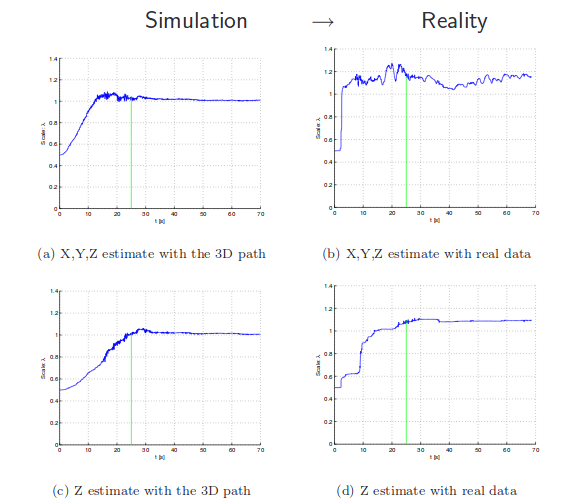
\includegraphics[width=\textwidth]{./figures/ekfTest.png}
% figure caption is below the figure
\caption{Offline simulation results with simulated and real data. Fewer directions (X,Y,Z) included in Kalman filter gives us a better estimate of $\lambda$.~\cite{nutzi2011fusion}}
\label{fig:ekf1}       % Give a unique label
\end{figure}

Figure~\ref{fig:ekf1} shows the scale estimation $\lambda(t)$ for a simulated 3D path on left and actual path on right. The standard deviation for the acceleration noise for simulation was chosen same as real data($\sigma_{SLAM} = 0.01, \sigma_{IMU} = 0.2 m/s^2$) with initial velocity and acceleration set to zero. Plots in Fig.~\ref{fig:ekf1}a and Fig.~\ref{fig:ekf1}c do not differ due to simulating the acceleration from the spline ideally in world frame. The estimate becomes more accurate when we use less number of directions (X,Y,Z).  Wrong measurements in acceleration influence $\lambda$ and make the scale estimation sensitive as seen in Fig.~\ref{fig:ekf1}b. Hence only using a single axis (Z-axis) gives us the best result. 


\subsubsection{Online Implementation}

For the online implementation, the third setup was incorporated into the PTAM code~\cite{ptamcode}. As mentioned in section~\ref{ptamtheory} PTAM employs two parallel threads called Tracker for tracking and MapMaker for mapping. Two additional threads for IMU and Kalman we added. The IMU thread provides the acceleration measurements. The Kalman thread starts with $\lambda$ calculated from integrating acceleration values, position from SLAM algorithm and acceleration and velocity set to 0. Values for covariance matrix \textbf{Q} is time-varied which provides control over the sensitivity of the Kalman filter. For our report we have not incorporated the online implementation and have reported results from the paper. 

% For one-column wide figures use
\begin{figure}
% Use the relevant command to insert your figure file.
% For example, with the graphicx package use
  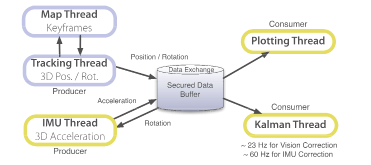
\includegraphics[width=\textwidth]{./figures/onlineEKF.png}
% figure caption is below the figure
\caption{Online implementation with PTAM work flow.Blue color boxes are original PTAM threads. Yellow boxes are added threads for scale estimation $\lambda$.~\cite{nutzi2011fusion}}
\label{fig:ekf2}       % Give a unique label
\end{figure}

\newpage
%\section{Introduction}
%\label{intro}
%Your text comes here. Separate text sections with
%\section{Section title}
%
%
%\label{sec:1}
%%Text with citations \cite{RefB} and \cite{RefJ}.
%\subsection{Subsection title}
%\label{sec:2}
%as required. Don't forget to give each section
%and subsection a unique label (see Sect.~\ref{sec:1}).
%\paragraph{Paragraph headings} Use paragraph headings as needed.
%\begin{equation}
%a^2+b^2=c^2
%\end{equation}
%
%% For one-column wide figures use
%\begin{figure}
%% Use the relevant command to insert your figure file.
%% For example, with the graphicx package use
%  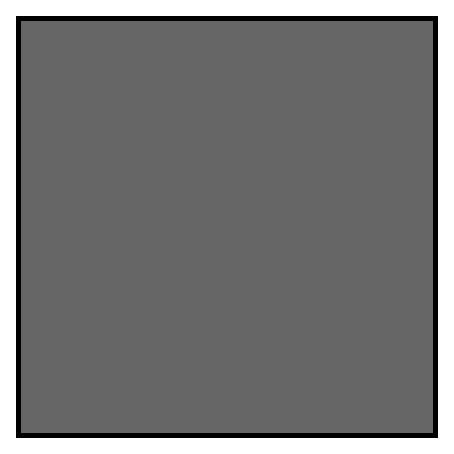
\includegraphics{example.eps}
%% figure caption is below the figure
%\caption{Please write your figure caption here}
%\label{fig:1}       % Give a unique label
%\end{figure}
%%
%% For two-column wide figures use
%\begin{figure*}
%% Use the relevant command to insert your figure file.
%% For example, with the graphicx package use
%  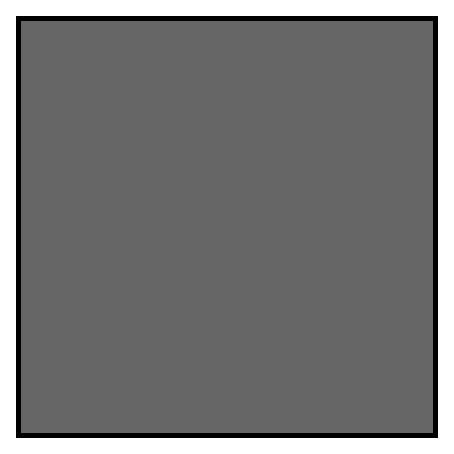
\includegraphics[width=0.75\textwidth]{example.eps}
%% figure caption is below the figure
%\caption{Please write your figure caption here}
%\label{fig:2}       % Give a unique label
%\end{figure*}
%%
%% For tables use
%\begin{table}
%% table caption is above the table
%\caption{Please write your table caption here}
%\label{tab:1}       % Give a unique label
%% For LaTeX tables use
%\begin{tabular}{lll}
%\hline\noalign{\smallskip}
%first & second & third  \\
%\noalign{\smallskip}\hline\noalign{\smallskip}
%number & number & number \\
%number & number & number \\
%\noalign{\smallskip}\hline
%\end{tabular}
%\end{table}

\nocite{*}

%\begin{acknowledgements}
%If you'd like to thank anyone, place your comments here
%and remove the percent signs.
%\end{acknowledgements}

% BibTeX users please use one of
\bibliographystyle{plain}
%\bibliographystyle{spbasic}      % basic style, author-year citations
%\bibliographystyle{spmpsci}      % mathematics and physical sciences
%\bibliographystyle{spphys}       % APS-like style for physics
\bibliography{references}   % name your BibTeX data base

%% Non-BibTeX users please use
%\begin{thebibliography}{}
%%
%% and use \bibitem to create references. Consult the Instructions
%% for authors for reference list style.
%%
%\bibitem{RefJ}
%% Format for Journal Reference
%Zhang, Zhengyou, Article title, Journal, Volume, page numbers (year)
%% Format for books
%\bibitem{RefB}
%%Author, Book title, page numbers. Publisher, place (year)
%% etc
%\end{thebibliography}

\end{document}
% end of file template.tex

